\section{Lineare Regression}
\index{Regression!lineare}
\index{lineare Regression}
\index{Kurvenanpassung}
\begin{figure}
\begin{center}
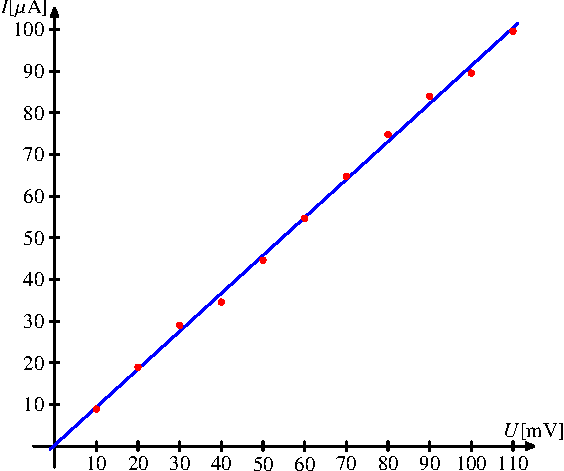
\includegraphics{images/regression-1.pdf}
\end{center}
\caption{Anpassung einer Geraden an gemessene
Strom-/Spannungswerte\label{ohm-regression}}
\end{figure}
Der Satz \ref{erwartungswert-charakterisierung} hat gezeigt, dass der
Erwartungswert jener Wert ist, der die Varianz minimiert.
Diese Idee
lässt sich auch auf kompliziertere Zusammenhänge anwenden.
In einem
Stromkreis erwartet man auf Grund des Ohmschen Gesetzes, dass Spannung $U$
und Strom $I$ proportional sind: $U=RI$.
Führt man eine Messung von beiden
Grössen durch, erhält man zwei Zufallsvariablen $U(\omega)$ und $I(\omega)$,
und die Proportionalität wird wegen der Messfehler meistens nicht mehr
erfüllt sein.
Wie gross ist der Widerstandswert $R$? Es wäre zwar denkbar,
für jede Messung den Widerstandswert zu errechnen, und dann das Mittel
zu bilden.
Noch besser ist aber, den Widerstandswert $R$ so zu bestimmen,
dass der erwartete quadratische Fehler
$E( (U-RI)^2)$
möglichst klein ist.
Abbildung \ref{ohm-regression} zeigt eine solche Gerade.


\subsection{Regressionsgerade}
Etwas allgemeiner finden wir folgenden Satz über die sogenannte
Regressionsgerade:
\begin{satz}
\label{rekursion}
Seien $X$ und $Y$ zwei reelle Zufallsvariablen.
Die Gerade mit der
Gleichung $y=ax+b$ minimiert die Varianz
$\operatorname{var}(aX+b-Y)$ genau dann, wenn 
\begin{align*}
a
&=
\frac{E(XY)-E(X)E(Y)}{(E(X^2)-E(X)^2)}=\frac{\operatorname{cov}(X,Y)}{\operatorname{var}(X)},
\\
b
&=
E(Y)-E(X)a.
\end{align*}
\end{satz}
\begin{proof}[Beweis]
Der mittlere quadratische Fehler ist
\begin{align*}
Q(a,b)&=E((aX+b-Y)^2)\\
&=E(a^2X^2+b^2+Y^2+2abX-2aXY -2bY)\\
&=a^2E(X^2)+b^2+E(Y^2)+2abE(X)-2aE(XY)-2bE(Y).
\end{align*}
Um das Minimum zu finden, setzen wir die partiellen Ableitungen nach $a$
und $b$ gleich Null, und finden:
\begin{align*}
0=\frac{\partial Q}{\partial a}&=2aE(X^2)+2bE(X)-2E(XY)\\
0=\frac{\partial Q}{\partial b}&=2b+2aE(X)-2E(Y).
\end{align*}
Dies ist gleichbedeutend mit dem folgenden linearen Gleichungssystem für
die Koeffizienten
$a$ und $b$
\begin{alignat*}{4}
E(X^2)a\,&+\,&E(X)b\,&=\,&E(XY)\\
E(X)a\,&+&b\,&=&E(Y).
\end{alignat*}
Multipliziert man die zweite Gleichung mit $E(X)$ und subtrahiert sie von der
ersten, erhält man eine Gleichung für $a$:
\begin{align*}
(E(X^2)-E(X)^2)a&=E(XY)-E(X)E(Y)\\
a&=\frac{E(XY)-E(X)E(Y)}{(E(X^2)-E(X)^2)}.
\end{align*}
Aus der zweiten Gleichung kann man nun auch $b$ finden:
\[
b=E(Y)-E(X)a,
\]
womit alles bewiesen ist.
\end{proof}
Die Gleichung für $b$ hat eine unmittelbare Konsequenz: die Regressionsgerade
geht immer durch den Punkt $(E(X), E(Y))$.
In der Tat, damit der Punkt
$(E(X), E(Y))$ auf der Geraden liegt, muss die Bedingung $E(Y)=aE(X)+b$
erfüllt sein.
Schafft man $aE(X)$ auf die linke Seite, wird daraus

$E(Y)-aE(X)=b$, also genau die Gleichung für $b$.

\subsubsection{Der mittlere quadratische Fehler}
Der mittlere quadratische Fehler lässt sich natürlich auch berechnen.
Wir sind von $\operatorname{var}(Y-aX-b)$ als zu optimierender
Grösse ausgegangen.
Inzwischen haben wir $a$ und $b$ bestimmt,
also können wir auch den Fehler berechnen.
Dazu sind die Rechenregeln
hilfreich:
\begin{align*}
\operatorname{var}(Y-aX-b)
&=
\operatorname{var}(Y) + 
\operatorname{var}(-aX) + 
\operatorname{var}(-b)
+2\operatorname{cov}(-aX,Y)
\\
&=
\operatorname{var}(Y)+a^2\operatorname{var}(X)-2a\operatorname{cov}(X,Y)
\\
&=
\operatorname{var}(Y)
+ \frac{\operatorname{cov}(X,Y)^2}{\operatorname{var}(X)^2}\operatorname{var}(X)
-2 \frac{\operatorname{cov}(X,Y)}{\operatorname{var}(X)}\operatorname{cov}(X,Y)
\\
&=
\operatorname{var}(Y)-\frac{\operatorname{cov}(X,Y)^2}{\operatorname{var}(X)}.
\end{align*}
Im zweiten Schritt mussten wir die Formel (\ref{var-summe-abhaengig})
verwenden, da die Zufallsvariablen $X$ und $Y$ nicht unabhängig sind.

Natürlich
ist der Fehler 
wahrscheinlich ungefähr proportional zur Varianz der $Y$-Werte,
ohne Varianz gibt's auch keinen Fehler.
Wir versuchen daher den Term
$\operatorname{var}(Y)$ auszuklammern:
\begin{align*}
\operatorname{var}(Y-aX-b)
&=
\operatorname{var}(Y)\left(1-\frac{\operatorname{cov}(X,Y)^2}{\operatorname{var}(X)\operatorname{var}(Y)}\right).
\end{align*}
Der Bruch wird damit ein natürliches Qualitätsmass für die Regressionsgerade:
\begin{definition}
Der Quotient
\[
r=\frac{\operatorname{cov}(X,Y)}{\sqrt{\operatorname{var}(X)\operatorname{var}(Y)}}
\]
heisst Regressionskoeffizient.
\end{definition}

\begin{figure}
\centering
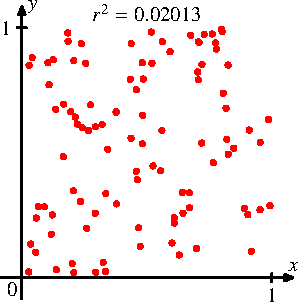
\includegraphics{images/regression-2.pdf}\;
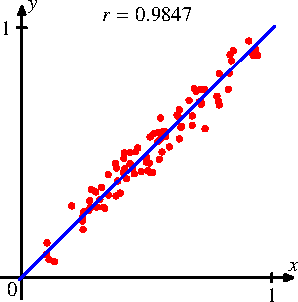
\includegraphics{images/regression-3.pdf}\;
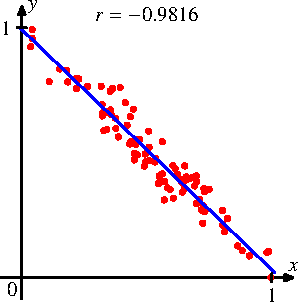
\includegraphics{images/regression-4.pdf}
\caption{Aussehen der Punktwolke für verschiedene Werte des Regressionskoeffizienten.
Für $r\simeq 0$ besteht keine Abhängigkeit zwischen den Variablen, $r\simeq 1$
zeigt eine gute, positive Abhängigkeit an, $r\simeq -1$ eine starke
negative Abhängigkeit.
\label{regressionskoeffizient-graphik}}
\end{figure}

Die Regression ist also umso genauer, je näher $r$ bei $\pm 1$ liegt.
Ausserdem hat $r$ immer das gleiche Vorzeichen wie die
Steigung der Regressionsgeraden.
Dies ist in Abbildung~\ref{regressionskoeffizient-graphik} dargestellt.

\subsubsection{Berechnung aus empirischen Daten}
Auch die Koeffizienten der Regressionsgeraden sind mit einfachen Formeln
zu bestimmen, wenn man nur Messwerte, deren Quadrate und das Produkt summiert:
\begin{align}
a
&=
\frac{\displaystyle n\sum_{i=1}^nx_iy_i-\sum_{i=1}^nx_i\sum_{i=1}^ny_i}{\displaystyle n\sum_{i=1}^nx_i^2-\biggl(\sum_{i=1}^nx_i\biggr)^2},
\label{lr:a}
\\
b
&=
\frac1n\sum_{i=1}^ny_i-a\frac1n\sum_{i=1}^nx_i,
\label{lr:b}
\\
r^2
&=
\frac{
\displaystyle
\biggl(n\sum_{i=1}^n x_iy_i-\sum_{i=1}^n x_i\sum_{i=1}^ny_i\biggr)^2
}{
\displaystyle
\biggl(n\sum_{i=1}^nx_i^2-\biggl(\sum_{i=1}^nx_i\biggr)^2\biggr)
\biggl(n\sum_{i=1}^ny_i^2-\biggl(\sum_{i=1}^ny_i\biggr)^2\biggr)
}.
\label{lr:r2}
\end{align}

\subsection{Anwendungsbeispiel}
\begin{table}
\begin{center}
\begin{tabular}{|c|c|}
\hline
Zeit [s]&Länge [mm]\\
\hline
6&10.98\\
10&13.89\\
14&16.23\\
18&18.57\\
\hline
\end{tabular}
\end{center}
\caption{Länge der Verzögerungselemente für K1100T in Abhängigkeit von der
Verzögerungszeit\label{delaylengths}}
\end{table}
Modellraketenmotoren auf Feststoffbasis verwenden ein Verzögerungselement,
welches nach Abbrand des eigentlichen Treibsstoffs noch einige Sekunden
weiter brennt, um dann eine Schwarzpulverladung zu zünden, die einen Fallschirm
auswerfen kann.
Die Verzögerungselemente werden nur für wenige, diskrete
Verzögerungszeiten hergestellt.
Ist kein passendes Verzögerungselement
verfügbar, muss
ein längeres Verzögerungselement durch Verkürzung auf die passende
Verzögerungszeit eingestellt werden.
Dazu muss jedoch der Zusammenhang
zwischen Verzögerungszeit und Länge des Elementes bekannt sein.
Der Hersteller macht die Angaben in Tabelle \ref{delaylengths}.

\subsubsection{Berechnung von Hand}
Die Berechnung auf dem Papier kann man zum Beispiel mit Hilfe
des Berechnungsschemas gemäss folgender Tabelle
organisieren, welche auch alle relevanten Formeln zeigt:
\begin{center}
\begin{tabular}{|l|l|l|l|}
\hline
$E(T)$&&&\\
$E(T^2)$&\footnotesize$\operatorname{var}(T)=E(T^2)-E(T)^2$&&\\
\hline
$E(L)$&&&\\
$E(L^2)$&\footnotesize$\operatorname{var}(L)=E(L^2)-E(L)^2$&&\\
\hline
$E(TL)$&\footnotesize$\operatorname{cov}(T,L)=E(TL)-E(T)E(L)$&$a=\frac{\operatorname{cov}(T,L)}{\operatorname{var}(T)}$&\footnotesize$b=E(L)-aE(T)$\\
&&$r=\frac{\operatorname{cov}(T,L)}{\sqrt{\operatorname{var}(T)\operatorname{var}(L)}}$&\\
\hline
\end{tabular}
\end{center}
Die Durchführung der Rechnung führt zu folgendem Resultat:
\begin{center}
\begin{tabular}{|r|r|r|r|}
\hline
12.0000&&&\\
164.0000&20.0000&&\\
\hline
14.9175&&&\\
230.4376&7.9058&&\\
\hline
191.5650&12.5550&0.627750&7.38450\\
&&0.998456&\\
\hline
\end{tabular}
\end{center}
Somit kann man als Näherungsformel für die Länge des Verzögerungselements
die lineare Funktion
\[
l=0.62775 \cdot t+7.3845
\]
verwenden.
Der mittlere quadratische Fehler dieser Näherung ist
\[
\Delta = \operatorname{var}(L)(1-r^2)=0.024.
\]
Der Längenfehler ist also etwa $\sigma_L=\sqrt{0.024}=0.15$mm, was einer
Ungenauigkeit der Verzögerungsdauer von 0.25s entspricht.
Angesichts
der Fertigungs- und Betriebs\-toleranzen von bis zu 20\%, verursacht durch
Schwankungen in Abmessungen, physikalischen Eigenschaften des Treibstoffs
und Temperatur beim Abbrand ist dies bei weitem genau genug.
\subsubsection{Berechnung mit R}
\begin{figure}
\begin{center}
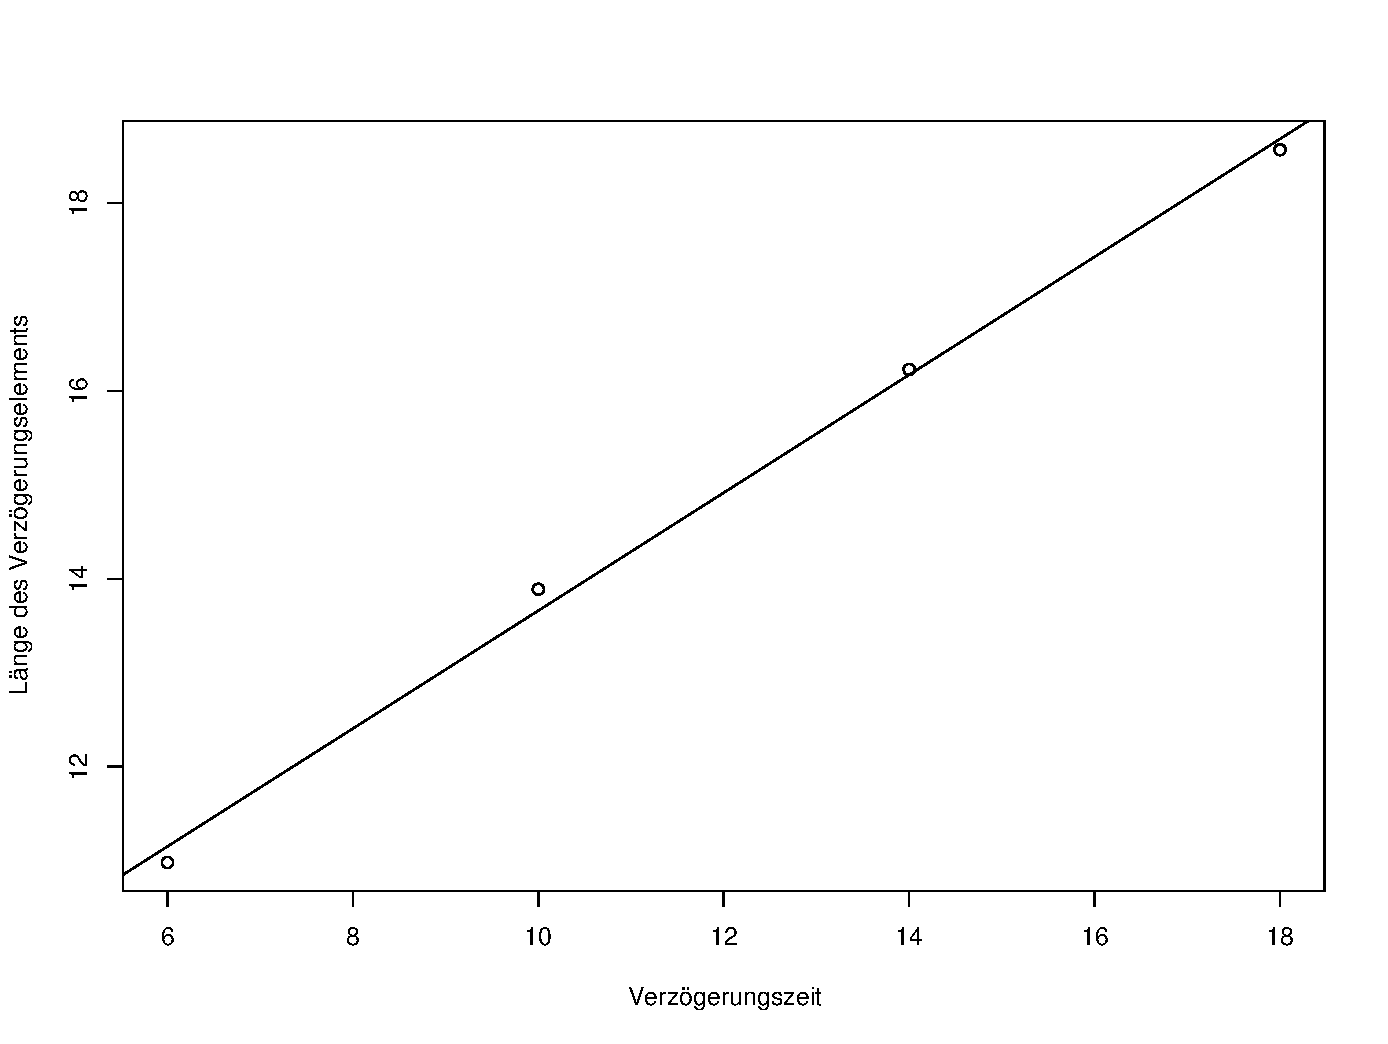
\includegraphics[width=0.7\hsize]{graphics/verzoegerungszeit}
\end{center}
\caption{Von R erzeugte graphische Darstellung der Regressionsgerade
für die Verzögerungszeit\label{verzoegerungszeit}}
\end{figure}
Die Software R
ist ein leistungsfähiges freies Softwarepaket für statistische
Berechnungen.
Mit folgenden Befehlen kann das obige Regressionsproblem
mit R gelöst, und die Graphik \ref{verzoegerungszeit} dargestellt
werden:

{\footnotesize
\begin{verbatim}
> zeit = c(6,10,14,18)
> laenge = c(10.98, 13.89, 16.23, 18.57)
> laenge.lm = lm(laenge ~ zeit)
> summary(laenge.lm)

Call:
lm(formula = laenge ~ zeit)

Residuals:
     1      2      3      4 
-0.171  0.228  0.057 -0.114 

Coefficients:
            Estimate Std. Error t value Pr(>|t|)   
(Intercept)  7.38450    0.31608   23.36  0.00183 **
zeit         0.62775    0.02468   25.43  0.00154 **
---
Signif. codes:  0 `***' 0.001 `**' 0.01 `*' 0.05 `â'0.1 ` ' 1 

Residual standard error: 0.2208 on 2 degrees of freedom
Multiple R-Squared: 0.9969,	Adjusted R-squared: 0.9954 
F-statistic: 646.9 on 1 and 2 DF,  p-value: 0.001542 

> plot(laenge ~ zeit, xlab="Verzoegerungszeit",
  ylab="Laenge des Verzoegerungselements")
> abline(laenge.lm)
\end{verbatim}
}
R kann von \url{https://www.r-project.org} heruntergeladen werden.

